\documentclass[12pt, a4paper]{book}%, oneside

\usepackage[headings]{fullpage}
\usepackage{setspace}

% \usepackage[top=1.5cm,right=1.5cm,bottom=1.5cm,left=1.5cm]{geometry}
% \usepackage{fancyhdr}
% \setlength{\headheight}{20pt} 
% \usepackage{graphics}
\usepackage{graphicx}
\usepackage{float}
\usepackage{subfig}
\usepackage{array}
% \usepackage{xtab}
\usepackage{multirow}
\usepackage{booktabs}
\usepackage{appendix}
\usepackage[pdfborder={0 0 0}, colorlinks=true, linkcolor=black, citecolor=blue]{hyperref}
\usepackage[printonlyused]{acronym}
\usepackage{algorithmic}
\usepackage{algorithm}
\usepackage{ifpdf}
% \setlength{\parindent}{0pt}

\newcommand{\submissionDay}{14}
\newcommand{\submissionMonth}{May}
\newcommand{\submissionYear}{2013}
\newcommand{\submissionDate}{\submissionDay~\submissionMonth,~\submissionYear}
\newcommand{\typeOfThesis}{Bachelor Thesis}

\newcommand{\titleOfThesisOne}{Virtual Arduino}

\newcommand{\authorOfThesis}{Ahmed Sabbah}
\newcommand{\supervisorOne}{Assoc. Prof. Georg Jung}
\newcommand{\supervisorTwo}{}
\newcommand{\supervisorThree}{}

\newcommand{\includefig}[4]{
    \begin{figure}[ht]
     \centering
      \includegraphics[width=#1\textwidth]{images/#2}
      \caption{#3}
      \label{#4}
    \end{figure}
}

\newcommand{\includefigWSC}[5]{
    \begin{figure}[ht]
     \centering
      \includegraphics[width=#1\textwidth]{images/#2}
      \caption[#3]{#4}
      \label{#5}
    \end{figure}
}

\newcommand{\includeeps}[4]{
\includefig{#1}{#2.eps}{#3}{#4}
}

\newcommand{\includeepsWSC}[5]{
\includefigWSC{#1}{#2.eps}{#3}{#4}{#5}
}


\ifpdf
\pdfinfo {
	/Author (\authorOfThesis)
	/Title (\titleOfThesisOne)
	/Subject (\typeOfThesis)
	/Keywords ()
	/CreationDate (D:20090707085533)
}
\fi

\begin{document}
% \overfullrule=5pt
\pagestyle{plain}
\pagenumbering{Roman}

\newcommand{\titlePage}{

\thispagestyle{empty}
\begin{center}
	\textbf{Media Engineering and Technology Faculty}\\[1mm]
	\textbf{German University in Cairo}\\[1mm]
	
\includegraphics[width=2.5cm]{GUC-logo-ss.eps}
	
	\vspace{2cm}
	\doublespacing
	{\Huge \textbf{\titleOfThesisOne}}\\
	\singlespacing
	\vspace{2cm}
	{\large \textbf{\typeOfThesis}}\\
	
	\vfill
	\parbox{1cm}{
  		\begin{large}
    			\begin{tabbing}
       			Author: \hspace{2cm}  
        			\=\authorOfThesis\\[2mm]
      			Supervisors: 
        			\>\supervisorOne\\[2mm]
				\>\supervisorTwo\\[2mm]
				\>\supervisorThree\\[2mm]
      			Submission Date: 
        			\>\submissionDate\\
    			\end{tabbing}
  		\end{large}
	}\\
\end{center}
\clearpage
}
%++++++++++++++++++++++++++++++++++++++++++++++++++++++++++++++++++++
\titlePage
\thispagestyle{empty}\ \clearpage
\titlePage
%++++++++++++++++++++++++++++++++++++++++++++++++++++++++++++++++++++
\thispagestyle{empty}
This is to certify that:
\begin{itemize}
\item[(i)] the thesis comprises only my original work toward the Bachelor Degree
\item[(ii)] due acknowlegement has been made in the text to all other material used
\end{itemize}

\vspace{2cm}
\begin{flushright}
\rule[0mm]{6cm}{0.2mm}\\
\authorOfThesis\\
\submissionDay~\submissionMonth,~\submissionYear\\
\end{flushright}
\clearpage


%\chapter*{Acknowledgments}
\addcontentsline{toc}{chapter}{Acknowledgments}
\label{chap:ack}
I would like to express my greatest gratitude to the people who have helped & supported me throughout my project. I am grateful to my supervisor Georg Jung for his continuous support for the project, from initial advice in the early stages of conceptual inception & through ongoing advice & encouragement to this day. 

A special thank of mine goes to my project partner Ahmed Sabbah who helped bring this idea to life.

I would also like to thank the Arduino developers community as they were extremely helpful and supportive. 
\clearpage  % Declaration ended, now start a new page

%% ----------------------------------------------------------------
% The "Funny Quote Page"
\pagestyle{empty}  % No headers or footers for the following pages

\null\vfill
% Now comes the "Funny Quote", written in italics
%\textit{``Write a funny quote here.''}

%\begin{flushright}
%If the quote is taken from someone, their name goes here
%\end{flushright}

\vfill\vfill\vfill\vfill\vfill\vfill\null
\clearpage  % Funny Quote page ended, start a new page
%% -------------------------------------------------------

\chapter*{Abstract}
% \addcontentsline{toc}{chapter}{Abstract}
\label{chap:abstract}

The use of microcontrollers is becoming more popular year by year. Nearly all devices now have microcontrollers. They even invented a \href{http://www.inquisitr.com/270421/goal-line-technology-being-tested-by-fifa-ifab/}{soccer ball with a built-in microchip}. Microcontroller boards are widely used for educational purposes in universities. they are considered an efficient way to learn and practice embedded systems programming, as it provides hands-on experience to the user. However, many university students do not have access to these boards as they are expensive. The challenge nowadays is to decrease this cost. we provide a real time simulator for a popular microcontroller board, the \href{http://arduino.cc/en/Main/ArduinoBoardUno}{Arduino Uno}. This simulator provides an experience as close as possible to the actual board. Using this simulator, the user can write Arduino code, compile and upload it to a simulated Arduino Uno board. He can also implement circuit simulators, add virtual hardware components and connect them to the virtual board. The simulator also provides visualization for the output that the Arduino board produces on the circuits and hardware components. Through this application, the user has the opportunity to learn most of the phases of working with microcontrollers.


\tableofcontents
% \addcontentsline{toc}{chapter}{Contents}
\clearpage 

\pagestyle{headings}
\pagenumbering{arabic}

% \setlength\parskip{15pt}
\setlength\parskip{.5\baselineskip plus .2\baselineskip
	minus .4\baselineskip}
% \setlength\parskip{.5\baselineskip \@plus .1\baselineskip \@minus ..1\baselineskip}


\chapter{Introduction}
\label{chap:intro}

A microcontroller is a small computer on a single integrated circuit containing a processor core, memory, and programmable input/output peripherals\cite{Wikidef:URL}. Arduino Uno is based on the \href{http://www.atmel.com/devices/atmega328.aspx?tab=overview}{ATmega328} microcontroller. It is a popular and easy to work with microcontroller board. We provide a simulation for Arduino Uno, ATmega328 microcontroller and the experience of working with them.

\section*{Motivation} \label{sec:s1}
In educational context, microcontroller boards are considered a practical way for learning and practising embedded systems programming. These boards provide the user with the opportunity to learn to program and implement hardware circuits. Cost is a problem that stands against the growing use of microcontrollers mainly in educational context. This problem results in the unavailability of these boards in many universities, thus a lot of students do not have access to them. Making a simulator for these board would be a solution for this problem. Several simulators for Arduino have been implemented, but none of them can replace the the real life experience of the actual board and hardware components.

\section*{Aim of the project}
The aim of this project is to provide a real time hardware simulator for a commonly used microcontroller board (Arduino Uno). This simulator is as close as possible to real experience where it covers all aspects of an embedded system. It gives the user the ability to work with hardware components, hardware interfacing, board setting, code compilation and uploading. The user will be able to write, compile and upload Arduino code using the Arduino IDE. He will be able to implement the circuitry and hardware components virtually and connect them to Arduino Uno virtual board. He can choose from a scalable library of the most common hardware components. The output of the code and hardware connections is reflected on the board and circuitry. By providing these aspects, users would not need to buy the actual board or any hardware components.

\chapter{Background}\label{chap:background}

Arduino is an open-source electronics prototyping platform based on flexible, easy-to-use hardware and software, retrieved from \href{http://arduino.cc/en/}{Arduino.cc}. The Arduino board is designed around the 8-bit Atmel AVR microcontroller. Its software is composed of a standard C-based programming language compiler and a boot loader that executes on the microcontroller.



\section{Program Specs}

\begin{figure}[h!]
\centering
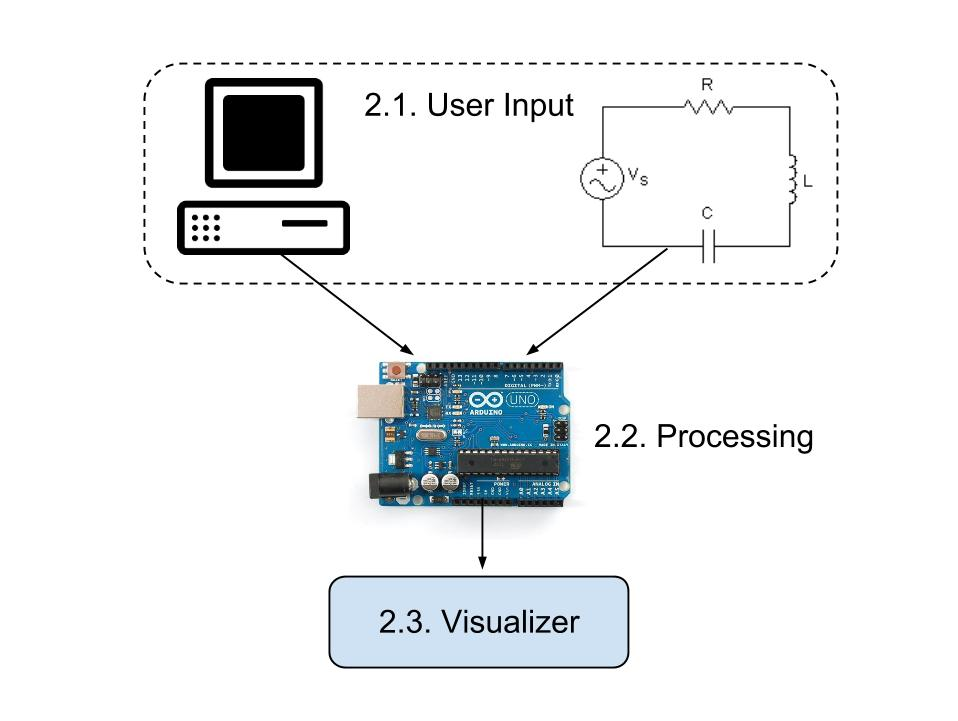
\includegraphics[height=9cm, width=12cm]{Hierarchy.jpg}
\caption{Virtual Arduino Architecture}
\label{Architecture}
\end{figure}
The following section will discuss the architectural hierarchy of the full program. The section will also partition the program into modules so it can be more easily conquered. 

\subsection{User Input}
The architecture is divided into three main parts, first part in the user input which can be in form  of text i.e Arduino code or in the form of circuitry.

\subsubsection{Computer Module}
Real-life Arduino system can be divided into two parts, Integrated development environment (IDE) and hardware. The IDE or Computer Module is where the user can write, compile and upload code onto the Arduino. This shall be implemented by using the already existing opensource Arduino IDE and redirecting its output to a virtual serial port so that this binary code can be later used for the simulation. This binary code will be transimitted down from user input to the processing module. Details about the computer mode internal workings shall be dicussed in sections 2.2 amd 2.3.

\subsubsection{Circuitry Module}
The second part of the Arduino experience is external hardware. One of the main advantages of the Arduino board is that it is easily interfaceable with most hardware components as it has built-in ADC and PWM. This module is where the user gets to experiment with hardware and connect with the Arduino board. The circuitry workspace should include an easily scalable hardware library and a circuit builder. The hardware components are divided into 3 types which are input, connectors and output. Input components are mainly sensors, connector components are wires and resistors and output components are LEDs and motors. We plan on implementing this part by using and already existing opensource simulator and upgrading its GUI and its hardware components to fit the concept of the Virtual Arduino. This will be done by adding some hardware failures scenarios and giving the simulator a more realistic GUI. The circuit output or simplification if I may say so will also be sent to the next level of the architecture for further processing and linking with Computer Module output. 

\subsection{Processing Module}
This module is the junction between the upper and lower level of the architecture. It takes the binary code from the Computer Module and translates it into actions in the Virtual Arduino processor. After evaluating the different internal components of the processor the Virtual Arduino output pins shall be assessed and this will reflect on the different output hardware components. The status of the different hardware components - whether high, low or PWM signal- shall be sent to the next level of the architecture which is the Visualizer.

\subsection{Visualizer}
This is the part where the user sees the output of his program. After the code is verified and is clear of any syntactic errors the user uploads the code onto his/her Virtual Arduino and output components start to show changes. The user will also be able to alter the environment by changing the input to the sensor and see the immediate change in the output components. 

\section{Bootloader}
\label{sec:bootloader}
\begin{figure}[h!]
\centering
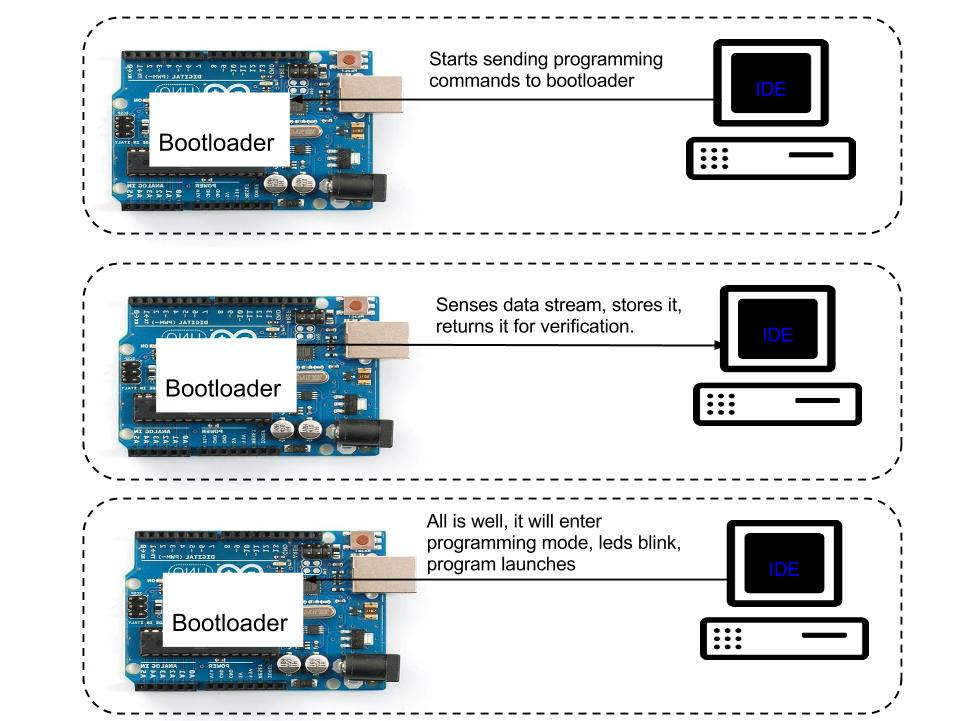
\includegraphics[height=9cm, width=12cm]{Bootloader.jpg}
\caption{Bootloader-Programmer Handshake}
\label{Bootloader Handshake}
\end{figure}
Stackoverflow \cite{Stackoverflow:URL} user \emph{angelatlarge} commented on April 3, 2013 (\href{http://stackoverflow.com/questions/15785087/upload-arduino-code-on-virtual-serial-port-through-arduino-ide/15792961?noredirect=1#comment22546153_15792961}{Upload Arduino code on virtual serial port through Arduino IDE}):
\begin{quotation}
``The process of uploading code is not a uni-directional process. There is a program on the Arduino called a bootloader [\emph{later discussed in section \ref{sec:bootloader}, the author}] which is responsible for communicating with the programmer (``programmer'': a program that programs the Arduino, assume it is the Arduino IDE for now). The Arduino CPUs cannot be programmed across serial lines. Rather these chips are programmed either via the \href{http://www.atmel.com/images/doc0943.pdf}{in system programming (ISP)} or via the \href{http://en.wikipedia.org/wiki/Jtag}{JTAG protocol}.
\end{quotation}
Retrieved from \href{http://stackoverflow.com/questions/15785087/upload-arduino-code-on-virtual-serial-port-through-arduino-ide/15792961?noredirect=1#comment22546153_15792961}{Stackoverflow}. 
Angelatlarge added  (2013, April 3).\href{http://stackoverflow.com/questions/15785087/upload-arduino-code-on-virtual-serial-port-through-arduino-ide/15792961?noredirect=1#comment22546153_15792961}{Upload Arduino code on virtual serial port through Arduino IDE} \begin{quotation}``The bootloader is a program that runs on the Arduino CPU, the program runs at startup and looks for programming commands over the serial port. If it discovers that a programmer is trying to communicate programming information, it will read the compiled Arduino binary coming over the serial link, store it in flash memory, send it back over the serial link for verification, and if everything is successful, exit and launch the stored sketch. If no programming information appears on the serial port, that is, no programmer is trying to write a new sketch, then the bootloader simply quits and launches the program already stored in flash.\end{quotation} Retrieved from http://stackoverflow.com/questions/15785087/upload-arduino-code-on-virtual-serial-port-through-arduino-ide/15792961?noredirect=1#comment22546153_15792961. 

Each Arduino board uses a different bootloader. In our program we will be simulating the ArduinoUno which uses the \href{https://github.com/arduino/Arduino/tree/master/hardware/arduino/bootloaders/optiboot}{optiboot bootloader} (publicly available on GitHub \cite{GitHub:URL}). Our plan is to mimic the responses sent from the bootloader to the IDE in order to get the code the is sent from the IDE to the flash on the Arduino board. The bootloader communicates with the IDE using the \href{http://www.atmel.com/Images/doc2525.pdf}{STK500 protocol}. The STK500 is a communication protocol of 8-bit AVR. The handshake in Figure 2.2 will also be discussed in further details in the next chapter.

\section{Communication}
In order to imitate the bootloader we had to sniff the serial port to understand what is being transmitted between the IDE and the board. First, the Programmer in the IDE tries to sync with a device so it sends an GETSYNC command ([30] [20]). If a device is connected, the bootloader replies with INSYC, OK ([14] [10]). See Figure \ref{STK_INSYNC}.
\begin{figure}[h!]
\centering
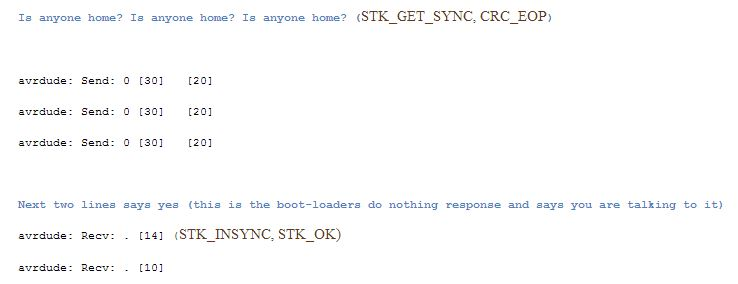
\includegraphics[height=7cm, width=16cm]{FirstStepSync.JPG}
\caption{SYNC with device}
\label{STK_INSYNC}
\end{figure}
After establishing the connection, the Programmer asks the bootloader about some of the board's specs such as the hardware, firmware, system clock and reference voltage. After setting the parameters, the IDE sends an ENTERPROGMODE command which tells the bootloader to program the chip. See Figure  \ref{ENTER_PROGMODE}.
\begin{figure}[h!]
\centering
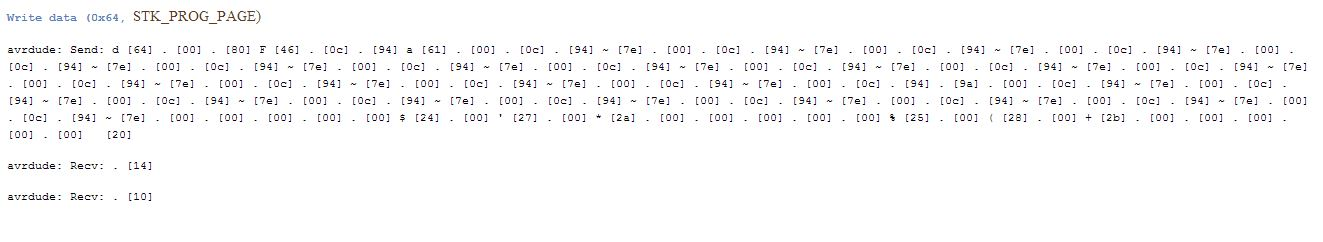
\includegraphics[height=9cm, width=17cm]{FirstChunckOfData.JPG}
\caption{First Chunk of Code}
\label{ENTER_PROGMODE}
\end{figure}
The code is sent from the IDE to the board and is written to the flash memory. But before programming the chip, this code has to be verified. The bootloader then sends back all what is on the flash for verification. After it is verified, the chip is programmed and the IDE tells the bootloader that it is done and sends a LEAVEPROGMODE command. See Figure  \ref{LEAVE_PROGMODE}.
\begin{figure}[h!]
\centering
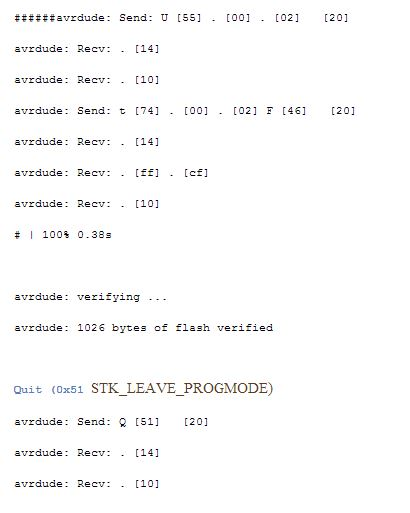
\includegraphics[height=20cm, width=16cm]{EndVarifyLeaveProgMode.JPG}
\caption{Verifies, End connection}
\label{LEAVE_PROGMODE}
\end{figure}

\section{Java Libraries}
To receive the Programmer's commands and respond to them like the bootloader, we had to communicate with our virtual serial port. There are several communication libraries in Java that offer such features. Sun had a serial communication API called JavaComm but they withdrew it's support for windows in 2005. This led to the development of the free open-source \href{http://rxtx.qbang.org/wiki/index.php/Main_Page}{RxTx library}. We chose to use the Java Simple Serial Connector \href{https://code.google.com/p/java-simple-serial-connector/}{(JSSC)} library which is based on the RxTx library.

\clearpage  % Introduction ended, start a new page


\chapter{Implementation}
\label{chap:implementation}

This module describes the core implementation of Arduino Uno. It is based on the ATmega328 microcontroller. The following is a block diagram that displays its components.



\begin{figure}[h!]
\centering
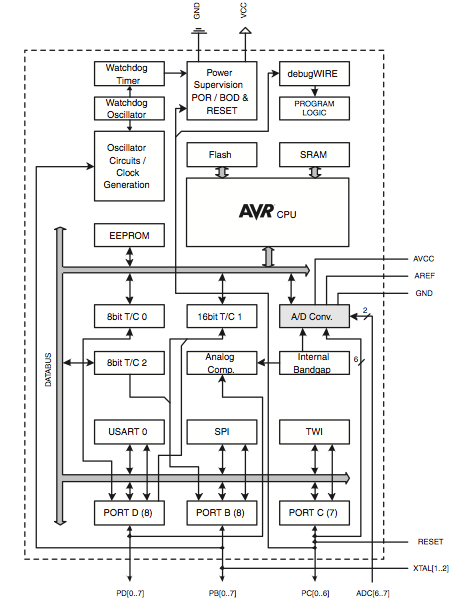
\includegraphics[height=12cm, width=10cm]{ArduinoBlockDiagram.png}
\caption{ATmega block diagram \protect\cite{BlockDiagram:URL}}
\label{Arduino Uno block diagram}
\end{figure}



\noindent \large The core implementation is divided into three main sections.

\section{Memory and registers}

In ATmega328, memory is divided into 3 main parts.
\subsection{Flash memory}
It is a non-volatile read only memory of 32 KB addressed by 15-bit addresses, 0.5 KB of them are used by bootloader. It is used for storing the program. 

\subsection{SRAM (data memory)}
It is a volatile memory of 2 KB. It is divided into 32 registers, 64 I/O registers, 160 external I/O registers and internal SRAM. See Figure \ref{SRAMcontents}.

\begin{figure}[h!]
\centering
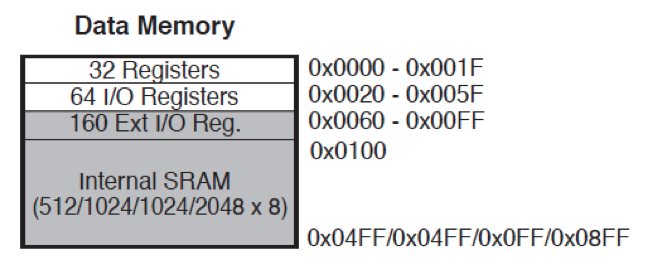
\includegraphics[height=4cm, width=9cm]{registers.png}
\caption{SRAM \protect\cite{WashUni:URL}}
\label{SRAMcontents}
\end{figure}

\newpage

\noindent The following are special registers saved in the SRAM 

\subsubsection{Program Status Register(PSR)}
It is a register for storing some status flags resulting from ALU operations. See Figure \ref{ProgramStatusRegister}.

\begin{figure}[h!]
\centering
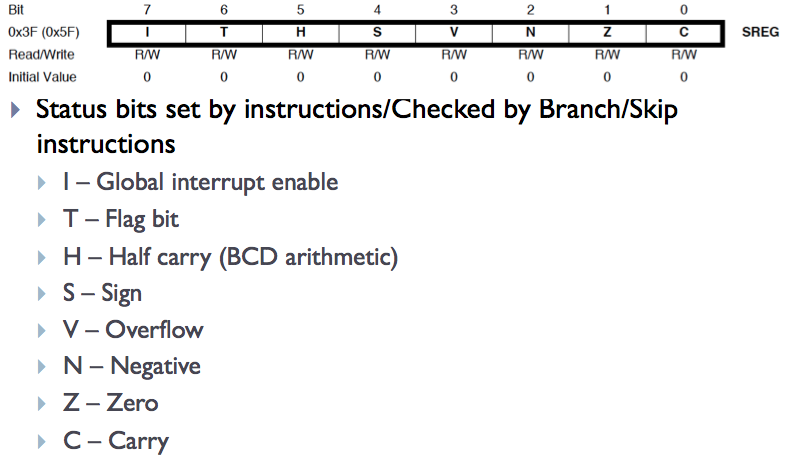
\includegraphics[height=7cm, width=12cm]{PSR.png}
\caption{Program Status Register \protect\cite{WashUni:URL}}
\label{ProgramStatusRegister}
\end{figure}

\subsubsection{Stack Pointer Register(SPR)}
It is a special register in I/O space that stores the address of the last program request in a stack.

\subsubsection{RAMPX, RAMPY, RAMPZ}
Registers concatenated with the X-, Y-, and Z-registers enabling indirect addressing of the whole data space on MCUs with more than 64K bytes data space, and constant data fetch on MCUs with more than 64K bytes program space. 
				
\subsubsection{RAMPD}
Register concatenated with the Z-register enabling direct addressing of the whole data space on MCUs with more than 64K bytes data space. 
	
\subsubsection{EIND}
Register concatenated with the Z-register enabling indirect jump and call to the whole program space on MCUs with more than 64K words (128K bytes) program space. 
				
\subsection{EEPROM}
It is a long term data memory of 1 KB.


\section{Reading program process}
This is the process of receiving bytes of code and saving their values in the flash memory to be ready for execution.

\section{Program execution}

This section describes the process of executing the program saved in the flash memory. ATmega328 is based on the \href{http://www.atmel.com/images/doc0856.pdf}{8-bit AVR Instruction Set}. An instruction can be either 16 or 32 bits. The application reads two bytes to form a 16 bit instruction (most significant bits first). For every instruction the opcode is matched and executed. See Figure \ref{InstructionOpcodeExample} for the ADD instruction opcode.

\begin{figure}[h!]
\centering
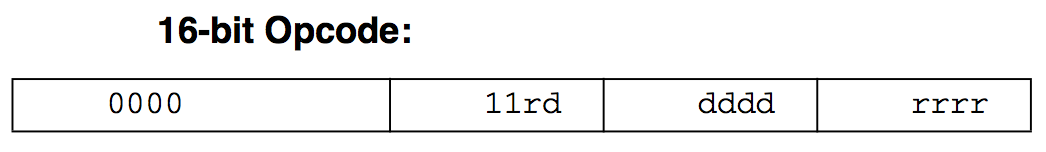
\includegraphics[height=1.5cm, width=10cm]{opcode.png}
\caption{ADD instruction opcode \protect\cite{opcode:URL}}
\label{InstructionOpcodeExample}
\end{figure}

To determine the opcode, bitwise operations are performed on the instruction. Opcodes for all instructions and their operation are found in the \href{http://www.atmel.com/images/doc0856.pdf}{AVR Instruction Set documentation}. After matching with an opcode, bitwise operations are performed to extract the operands from the instruction. Then comes the next part of executing the matched instruction according to the opcode.
\noindent Instruction might match with a 32 bit opcode which requires reading the next two bytes to extract the operand.






% \chapter{Conclusion}\label{chap:concl}


Hands-on experience is essential for students learning embedded system programming. Some students do not have access to microcontroller boards because of cost. A real time hardware simulation including all aspects of embedded system is a perfect solution to this problem. Students that use this application can gain most of the experience. They can write code, implement circuits and connect hardware components covering all aspect of embedded system programing.
% \chapter{Future Work}
\label{chap:todo}
Text

\appendix
\renewcommand{\appendixtocname}{Appendix}
\renewcommand{\appendixpagename}{\appendixtocname}
\addappheadtotoc
\setboolean{@twoside}{false}
\appendixpage

\chapter{Lists}
\addcontentsline{toc}{section}{List of Abbreviations}
\begin{acronym}[\hspace{3cm}]
  \acro{ac}[AC]{Acronym Without Citation}
  \acro{ac2}[AC2]{Acronym With Citation \cite{citeKey2}}
\end{acronym}
\clearpage
\listoffigures
\addcontentsline{toc}{section}{List of Figures}
% \listoftables
% \addcontentsline{toc}{section}{List of Tables}


\bibliographystyle{plain}
\bibliography{bachelor}
\addcontentsline{toc}{chapter}{References}

\end{document}
